\documentclass[frames]{prosper}
\title{Numerical Solutions of the 2-D Navier-Stokes Equations}
\author{Marvin Washington}
\institution{Jackson State University}
\begin{document}
\maketitle
\begin{slide}[Wipe]{Deformation of the Body}
\begin{figure}
\begin{center}
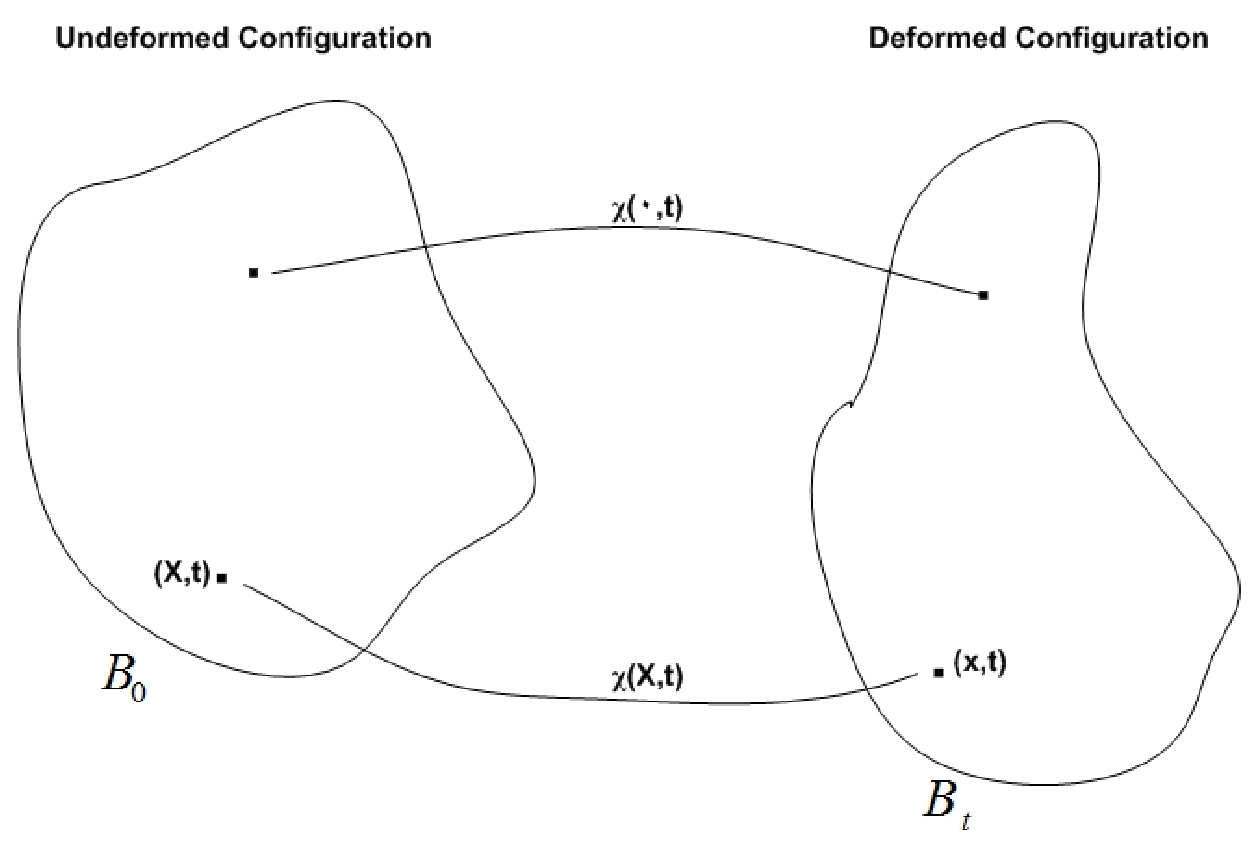
\includegraphics[scale = .3]{config_gragh_marvin.eps}
\end{center}
\end{figure}
\end{slide}

\begin{slide}[Box]{Reynold's Transport Theorem}
Let $V$ be a subset of the deformed configuration, and let $V_{0}$ be a subset of the undeformed configuration. Then for a differentiable function $f$ with continuous partial derivatives, we have
$$\frac{D}{Dt} \int_{V} f(\stackrel{\rightarrow}{x},t)dV = \int_{V}\left\{ {\frac{\partial f}{\partial t} + \nabla\cdot(f\stackrel{\rightarrow}{u})}\right\}dV$$
\end{slide}

\begin{slide}[Box]{Reynold's Transport Theorem Cont.}
\textbf{Proof.}
\begin{eqnarray*}
 \frac{D}{Dt} \int_{V} f(\stackrel{\rightarrow}{x},t)dV &=& \frac{D}{Dt} \int_{V_{0}} f(\chi(\textbf{X},t),t)J_{\chi}dV_{0}\\ \\
 &=& \int_{V_{0}}\left\{\frac{Df(\chi(\textbf{X},t),t)}{Dt}J_{\chi} + f(\chi(\textbf{X},t),t)\frac{DJ_{\chi}}{Dt}\right\}dV_{0}\\ \\ 
 &=& \int_{V_{0}}\left\{\frac{Df(\chi(\textbf{X},t),t)}{Dt}J_{\chi} + f(\chi(\textbf{X},t),t)J_{\chi}\nabla v\right\}dV_{0}\\ \\
 &=& \int_{V_{0}}\left\{\frac{Df(\chi(\textbf{X},t),t)}{Dt} + f(\chi(\textbf{X},t),t)\nabla v\right\}J_{\chi}dV_{0}\\ \\
 \end{eqnarray*}
\end{slide}

\begin{slide}[Box]{Reynold's Transport Theorem Cont.}
\begin{eqnarray*}
 &=& \int_{V_{0}}\left\{\frac{\partial f(\chi(\textbf{X},t),t)}{\partial t} + v\cdot \nabla f(\chi(\textbf{X},t),t) + f(\chi(\textbf{X},t),t)\cdot \nabla v\right\}J_{\chi}dV_{0}\\ \\
 &=& \int_{V}\left\{\frac{\partial f(\stackrel{\rightarrow}{x},t)}{\partial t} + \mbox{div}(f(\stackrel{\rightarrow}{x},t)v)\right\}dV\\ \\
\end{eqnarray*}
\end{slide}

\begin{slide}[Box]{Conservation of Mass}
The mass of a fluid $(M_{fluid})$ is given by the integral of the fluid density over the fluid domain i.e. $$ M_{fluid} = \int_{V} \rho(\stackrel{\rightarrow}{x},t)dV $$
The Conservation of Mass principle states that the derivative of mass w.r.t time must vanish i.e. $$ \frac{D}{Dt} \int_{V} \rho(\stackrel{\rightarrow}{x},t)dV = 0. $$
\end{slide}

\begin{slide}[Split]{Conservation of Mass Cont.}
Applying Reynold's Transport Theorem, we have $$ \frac{D}{Dt} \int_{V} \rho(\stackrel{\rightarrow}{x},t)dV = \int_{V} \left\{\frac{\partial \rho}{\partial t} + \nabla \cdot(\rho \stackrel{\rightarrow}{u})\right\}dV = 0. $$ Since we are working within the confines of the continuum hypothesis and since this equation must hold true for arbitrarily small domains, we can infer that $$ \frac{\partial \rho}{\partial t} + \nabla \cdot(\rho \stackrel{\rightarrow}{u}) = 0.$$ which is the continuity equation for compressible flows.
\end{slide}

\begin{slide}[Dissolve]{Conservation of Mass Cont.}
$$\frac{D\rho}{Dt} + \rho \nabla \cdot \stackrel{\rightarrow}{u} = 0.$$
which is the continuity equation for compressible flows.\\
in the case where the density remains constant $$\nabla \cdot \stackrel{\rightarrow}{u} = 0$$
is the continuity equation for incompressible flows.
\end{slide}



\begin{slide}[Dissolve]{Conservation of Momentum}
The Conservation of Linear Momentum Principle states that the rate of change of momentum w.r.t time is equal to the sum of the acting forces.
i.e.
$$ \frac{D}{Dt} \int_{V} \rho(\stackrel{\rightarrow}{x},t) \stackrel{\rightarrow}{u}dV = \sum \mbox{acting forces}$$
\end{slide}

\begin{slide}[Dissolve]{Conservation of Momentum Cont.}
Body forces will be expressed as $$ \int_{V} \rho(\stackrel{\rightarrow}{x},t) g(\stackrel{\rightarrow}{x},t)dV $$ and surface forces will be expressed as $$ \int_{\partial V} \sigma(\stackrel{\rightarrow}{x},t)\stackrel{\rightarrow}{n}ds $$
Recasting Newton's $2^{\mbox{nd}}$ law with this in mind yields $$ \frac{D}{Dt} \int_{V} \rho(\stackrel{\rightarrow}{x},t) \stackrel{\rightarrow}{u}dV = \int_{V} \rho(\stackrel{\rightarrow}{x},t) g(\stackrel{\rightarrow}{x},t)dV + \int_{\partial V} \sigma(\stackrel{\rightarrow}{x},t)\stackrel{\rightarrow}{n}ds $$
\end{slide}

\begin{slide}[Dissolve]{Conservation of Momentum Cont.}
Applying Reynold's Transport Theorem to the term on the left yields $$ \int_{V} \left\{\frac{\partial \rho \stackrel{\rightarrow}{u}}{\partial t} + \nabla \cdot \rho \stackrel{\rightarrow}{u}\stackrel{\rightarrow}{u}\right\}dV = \int_{V} \rho(\stackrel{\rightarrow}{x},t) g(\stackrel{\rightarrow}{x},t)dV + \int_{\partial V} \sigma(\stackrel{\rightarrow}{x},t)\stackrel{\rightarrow}{n}ds $$
After applying the Divergence Theorem to the last term and regrouping the equation we arrive at $$ \frac{\partial \rho \stackrel{\rightarrow}{u}}{\partial t} + (\stackrel{\rightarrow}{u} \cdot \nabla)\rho\stackrel{\rightarrow}{u} + \rho\stackrel{\rightarrow}{u}\nabla \cdot \stackrel{\rightarrow}{u} - \rho \stackrel{\rightarrow}{g} - \nabla \cdot \sigma = 0 $$
\end{slide}

\begin{slide}[Dissolve]{Conservation of Momentum Cont.}
The stress tensor $\sigma$ for viscous fluids is defined as $$ \sigma := -pI + \tau := -p + \lambda \mbox{div}(\stackrel{\rightarrow}{u})I + 2\mu\delta. $$ Using this stress tensor, the momentum equation becomes $$ \frac{\partial \rho \stackrel{\rightarrow}{u}}{\partial t} + (\stackrel{\rightarrow}{u} \cdot \nabla)\rho\stackrel{\rightarrow}{u} + \rho\stackrel{\rightarrow}{u}\nabla\cdot \stackrel{\rightarrow}{u} + \nabla p = (\mu + \lambda)\nabla(\mbox{div}(\stackrel{\rightarrow}{u})) + \mu\Delta\stackrel{\rightarrow}{u} + \rho\stackrel{\rightarrow}{g} $$

If the fluid being studied is incompressible(i.e $\rho$ = $\rho_{\infty}$ = constant), the momentum equation reduces to $$ \frac{\partial \stackrel{\rightarrow}{u}}{\partial t} + (\stackrel{\rightarrow}{u} \cdot \nabla)\stackrel{\rightarrow}{u} + \frac{1}{\rho_{\infty}}\nabla p = \frac{\mu}{\rho_{\infty}}\Delta\stackrel{\rightarrow}{u} + \stackrel{\rightarrow}{g} $$
\end{slide}

\begin{slide}[Dissolve]{Conservation of Momentum Cont.}
\begin{eqnarray*}
\left \{
\begin{array}{l r}
\displaystyle{\frac{\partial \stackrel{\rightarrow}{u}}{\partial t} + (\stackrel{\rightarrow}{u} \cdot \nabla)\stackrel{\rightarrow}{u} + \frac{1}{\rho_{\infty}}\nabla p = \frac{\mu}{\rho_{\infty}}\Delta\stackrel{\rightarrow}{u} + \stackrel{\rightarrow}{g}}\\
\nabla \cdot \stackrel{\rightarrow}{u} = 0 &
\end{array}
\right. 
\end{eqnarray*}
This system of equation is known as the Dimensional Navier-Stokes Equations for Incompressible Flow
\end{slide}

\begin{slide}[Dissolve]{Dimensional Analysis}
We obtain a dimensionless quantity by taking the ratio of the dimensional quantity over the reference quantity with the same unit.
Those variable are $\stackrel{\rightarrow}{u}$,$\stackrel{\rightarrow}{x}$,$p$,and $t$ and the associated reference quantities are $V$,$L$,$\rho_{\infty}V^2$, and $\displaystyle{\frac{L}{V}}$.
the dimensionless quantities can be defined as $$\stackrel{\rightarrow}{u}^* := \frac{\stackrel{\rightarrow}{u}}{V}, \stackrel{\rightarrow}{x}^* := \frac{\stackrel{\rightarrow}{x}}{L}, p^* := \frac{p}{\rho_{\infty}V^2}, t^* := \frac{Vt}{L}$$
\end{slide}

\begin{slide}[Dissolve]{Dimensional Analysis Cont.}
Substituting  these new variables into the momentum equation for incompressible flow yields
$$\frac{V^2}{L}\frac{\partial \stackrel{\rightarrow}{u}^*}{\partial t^*} + \frac{V^2}{L}(\stackrel{\rightarrow}{u}^* \cdot \mbox{grad}^*)\stackrel{\rightarrow}{u}^* + \frac{V^2}{L}\mbox{grad}^* p^* = \frac{V\mu}{L{^2}\rho_{\infty}} \Delta^* \stackrel{\rightarrow}{u}^* + \stackrel{\rightarrow}{g}$$
Multiplying through by $\displaystyle{\frac{L}{V^2}}$ yields, $$\frac{\partial \stackrel{\rightarrow}{u}^*}{\partial t^*} + (\stackrel{\rightarrow}{u}^* \cdot \mbox{grad}^*)\stackrel{\rightarrow}{u}^* + \mbox{grad}^* p^* = \frac{\mu}{L\rho_{\infty}V} \Delta^* \stackrel{\rightarrow}{u}^* + \frac{L}{V^2} \stackrel{\rightarrow}{g}$$
\end{slide}

\begin{slide}[Dissolve]{Dimensional Analysis Cont.}
This change of variable introduces two dimensionless quantities which describe properties of the flow
$$Re = \frac{\rho_{\infty}VL}{\mu} \Leftrightarrow \frac{\mbox{inertial forces}}{\mbox{viscous forces}}$$\\
$$Fr = \frac{V}{\sqrt{gL}} \Leftrightarrow \frac{\mbox{inertial forces}}{\mbox{gravitational forces}}$$
\end{slide}

\begin{slide}[Dissolve]{Dimensional Analysis Cont.}
With the introduction of the dimensionless body force $$ \stackrel{\rightarrow}{g^{*}} := \frac{L \stackrel{\rightarrow}{g}}{V^2} = \frac{1}{Fr^2}\frac{\stackrel{\rightarrow}{g}}{\left\|\stackrel{\rightarrow}{g}\right\|} $$ the equation becomes $$ \frac{\partial \stackrel{\rightarrow}{u}^*}{\partial t^*} + (\stackrel{\rightarrow}{u}^* \cdot \mbox{grad}^*)\stackrel{\rightarrow}{u}^* + \mbox{grad}^* p^* = \frac{\mu}{L\rho_{\infty}V} \Delta^* \stackrel{\rightarrow}{u}^* + \stackrel{\rightarrow}{g^{*}} $$
\end{slide}

\begin{slide}[Dissolve]{Dimensional Analysis Cont.}
Droping the * and rewriting the equations yields
\begin{eqnarray*}
\left \{
\begin{array}{l r}
\displaystyle{\frac{\partial \stackrel{\rightarrow}{u}}{\partial t} + (\stackrel{\rightarrow}{u} \cdot \nabla)\stackrel{\rightarrow}{u} + \nabla p = \frac{1}{Re}\Delta\stackrel{\rightarrow}{u} + \stackrel{\rightarrow}{g}}\\
\nabla \cdot \stackrel{\rightarrow}{u} = 0 &
\end{array}
\right. 
\end{eqnarray*}
This system of equation is known as the Dimensionless Navier-Stokes Equations for a Newtonian and Viscous Incompressible Flow
\end{slide}


\begin{slide}[Dissolve]{Finite-Difference Approximations}
$$ (u_{t})_{i}^{j} \approx \frac{u_{i}^{j+1} - u_{i}^{j}}{\delta t} $$ (forward finite difference approximation)
$$ (u_{t})_{i}^{j} \approx \frac{u_{i}^{j} - u_{i}^{j-1}}{\delta t} $$ (backward finite difference approximation)
$$ (u_{t})_{i}^{j} \approx \frac{u_{i}^{j+1} - u_{i}^{j-1}}{2\delta t} $$ (central finite difference approximation)
\end{slide}

\begin{slide}[Dissolve]{Finite-Difference Approximations}
\begin{figure}
\begin{center}
\caption{Staggered Grid}
\label{sg}
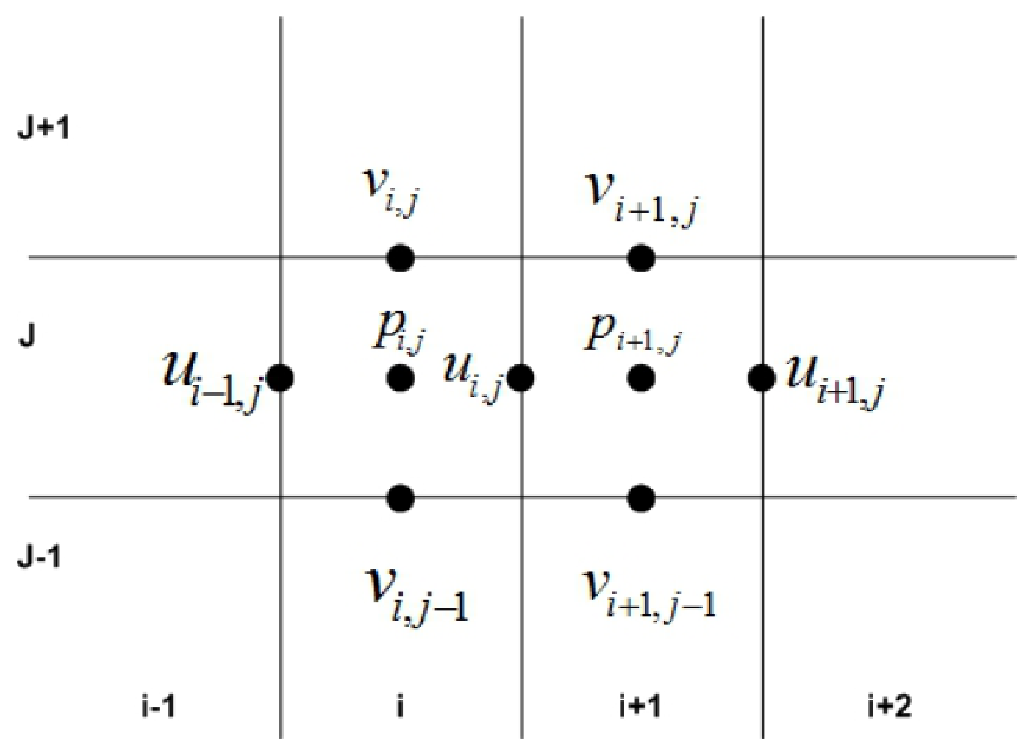
\includegraphics[scale = .3]{staggered_grid_marvin.eps}
\end{center}
\end{figure}
\end{slide}

\begin{slide}[Dissolve]{Finite-Difference Approximations}
$$\left[\frac{\partial u}{\partial t}\right]^{(n+1)} := \frac{u^{(n+1)} - u^{(n)}}{\delta t}, \hspace{.5in} \left[\frac{\partial v}{\partial t}\right]^{(n+1)} := \frac{v^{(n+1)} - v^{(n)}}{\delta t}$$
\end{slide}

\begin{slide}[Dissolve]{Finite-Difference Approximations}
$$u^{(n+1)} = u^{(n)} + \delta t\left[\frac{1}{Re}\left(\frac{\partial^2 u}{\partial x^2} + \frac{\partial^2 u}{\partial y^2}\right) - \frac{\partial (u^2)}{\partial x} - \frac{\partial (uv)}{\partial y} + g_{x} - \frac{\partial p}{\partial x}\right]$$\\

$$v^{(n+1)} = v^{(n)} + \delta t\left[\frac{1}{Re}\left(\frac{\partial^2 v}{\partial x^2} + \frac{\partial^2 v}{\partial y^2}\right) - \frac{\partial (uv)}{\partial x} - \frac{\partial (v^2)}{\partial y} + g_{y} - \frac{\partial p}{\partial y}\right]$$
\end{slide}


\begin{slide}[Dissolve]{Finite-Difference Approximations}
$$F := u^{(n)} + \delta t\left[\frac{1}{Re}\left(\frac{\partial^2 u}{\partial x^2} + \frac{\partial^2 u}{\partial y^2}\right) - \frac{\partial (u^2)}{\partial x} - \frac{\partial (uv)}{\partial y} + g_{x}\right]^{(n)}$$\\

$$G := v^{(n)} + \delta t\left[\frac{1}{Re}\left(\frac{\partial^2 v}{\partial x^2} + \frac{\partial^2 v}{\partial y^2}\right) - \frac{\partial (uv)}{\partial x} - \frac{\partial (v^2)}{\partial y} + g_{y}\right]^{(n)}$$
\end{slide}

\begin{slide}[Dissolve]{Finite-Difference Approximations}
$$u^{(n+1)} = F^{(n)} - \delta t \frac{\partial p^{(n+1)}}{\partial x}$$ 
$$v^{(n+1)} = G^{(n)} - \delta t \frac{\partial p^{(n+1)}}{\partial y}$$
Substitution into the continuity equation yields
$$\frac{\partial u^{(n+1)}}{\partial x} + \frac{\partial v^{(n+1)}}{\partial y} = \frac{\partial F^{(n)}}{\partial x} - \delta t \frac{\partial^2 p^{(n+1)}}{\partial x^2} + \frac{\partial G^{(n)}}{\partial y} - \delta t \frac{\partial^2 p^{(n+1)}}{\partial y^2} = 0$$
$$\frac{\partial^2 p^{(n+1)}}{\partial x^2} + \frac{\partial^2 p^{(n+1)}}{\partial y^2} = \frac{1}{\delta t} \left(\frac{\partial F^{(n)}}{\partial x} + \frac{\partial G^{(n)}}{\partial y}\right)$$
\end{slide}

\begin{slide}[Dissolve]{Donor-Cell Scheme}
The donor-cell discretization of some convective term $\displaystyle{\frac{d(ku)}{dx}}$ is defined by
$$\left[\frac{d(ku)}{dx}\right]_{i}^{dc} := \frac{k_{r}u_{r} - k_{l}u_{l}}{\delta x}$$
\end{slide}


\begin{slide}[Dissolve]{Donor-Cell Scheme}
$$ u_r := \left \{
\begin{array}{l r}
u_i & k_r > 0\\
u_{i+1} & k_r < 0
\end{array}
\right. \hspace{1in}
u_l := \left \{
\begin{array}{l r}
u_{i-1} & k_l > 0\\
u_{i} & k_l < 0
\end{array}
\right.$$
To avoid case distinctions, this can be written as
$$\left[\frac{d(ku)}{dx}\right]_{i}^{dc} := \frac{1}{2\delta x}\left(k_{r}(u_{i} + u_{i+1}) - k_{l} (u_{i-1} + u_{i}) + \left|k_{r}\right|(u_{i} - u_{i+1})$$
$$ - \left|k_{l}\right|(u_{i-1} - u_{i})\right)$$
\end{slide}


%\begin{slide}[Dissolve]{Finite-Difference Approximations}
%\end{slide}



\begin{slide}[Dissolve]{Flow in a Lid-Driven Cavity}
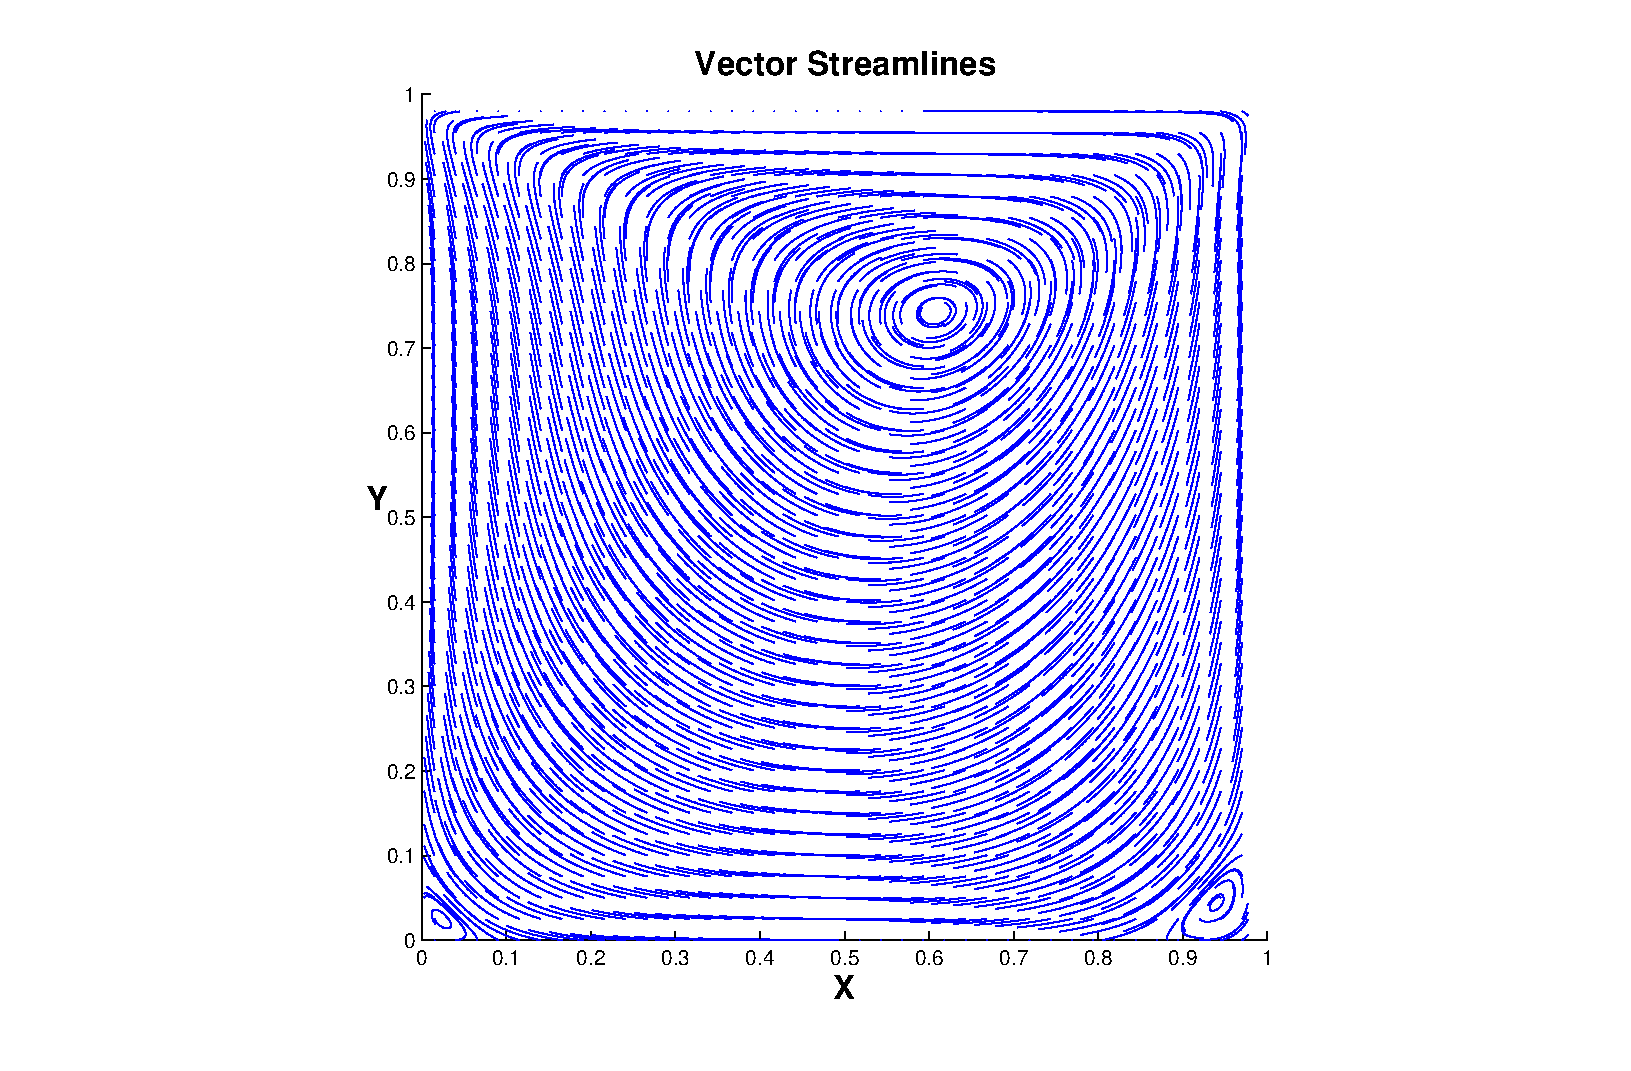
\includegraphics[scale=.4]{dcavity.eps}
\end{slide}

\begin{slide}[Dissolve]{Flow in a Lid-Driven Cavity}
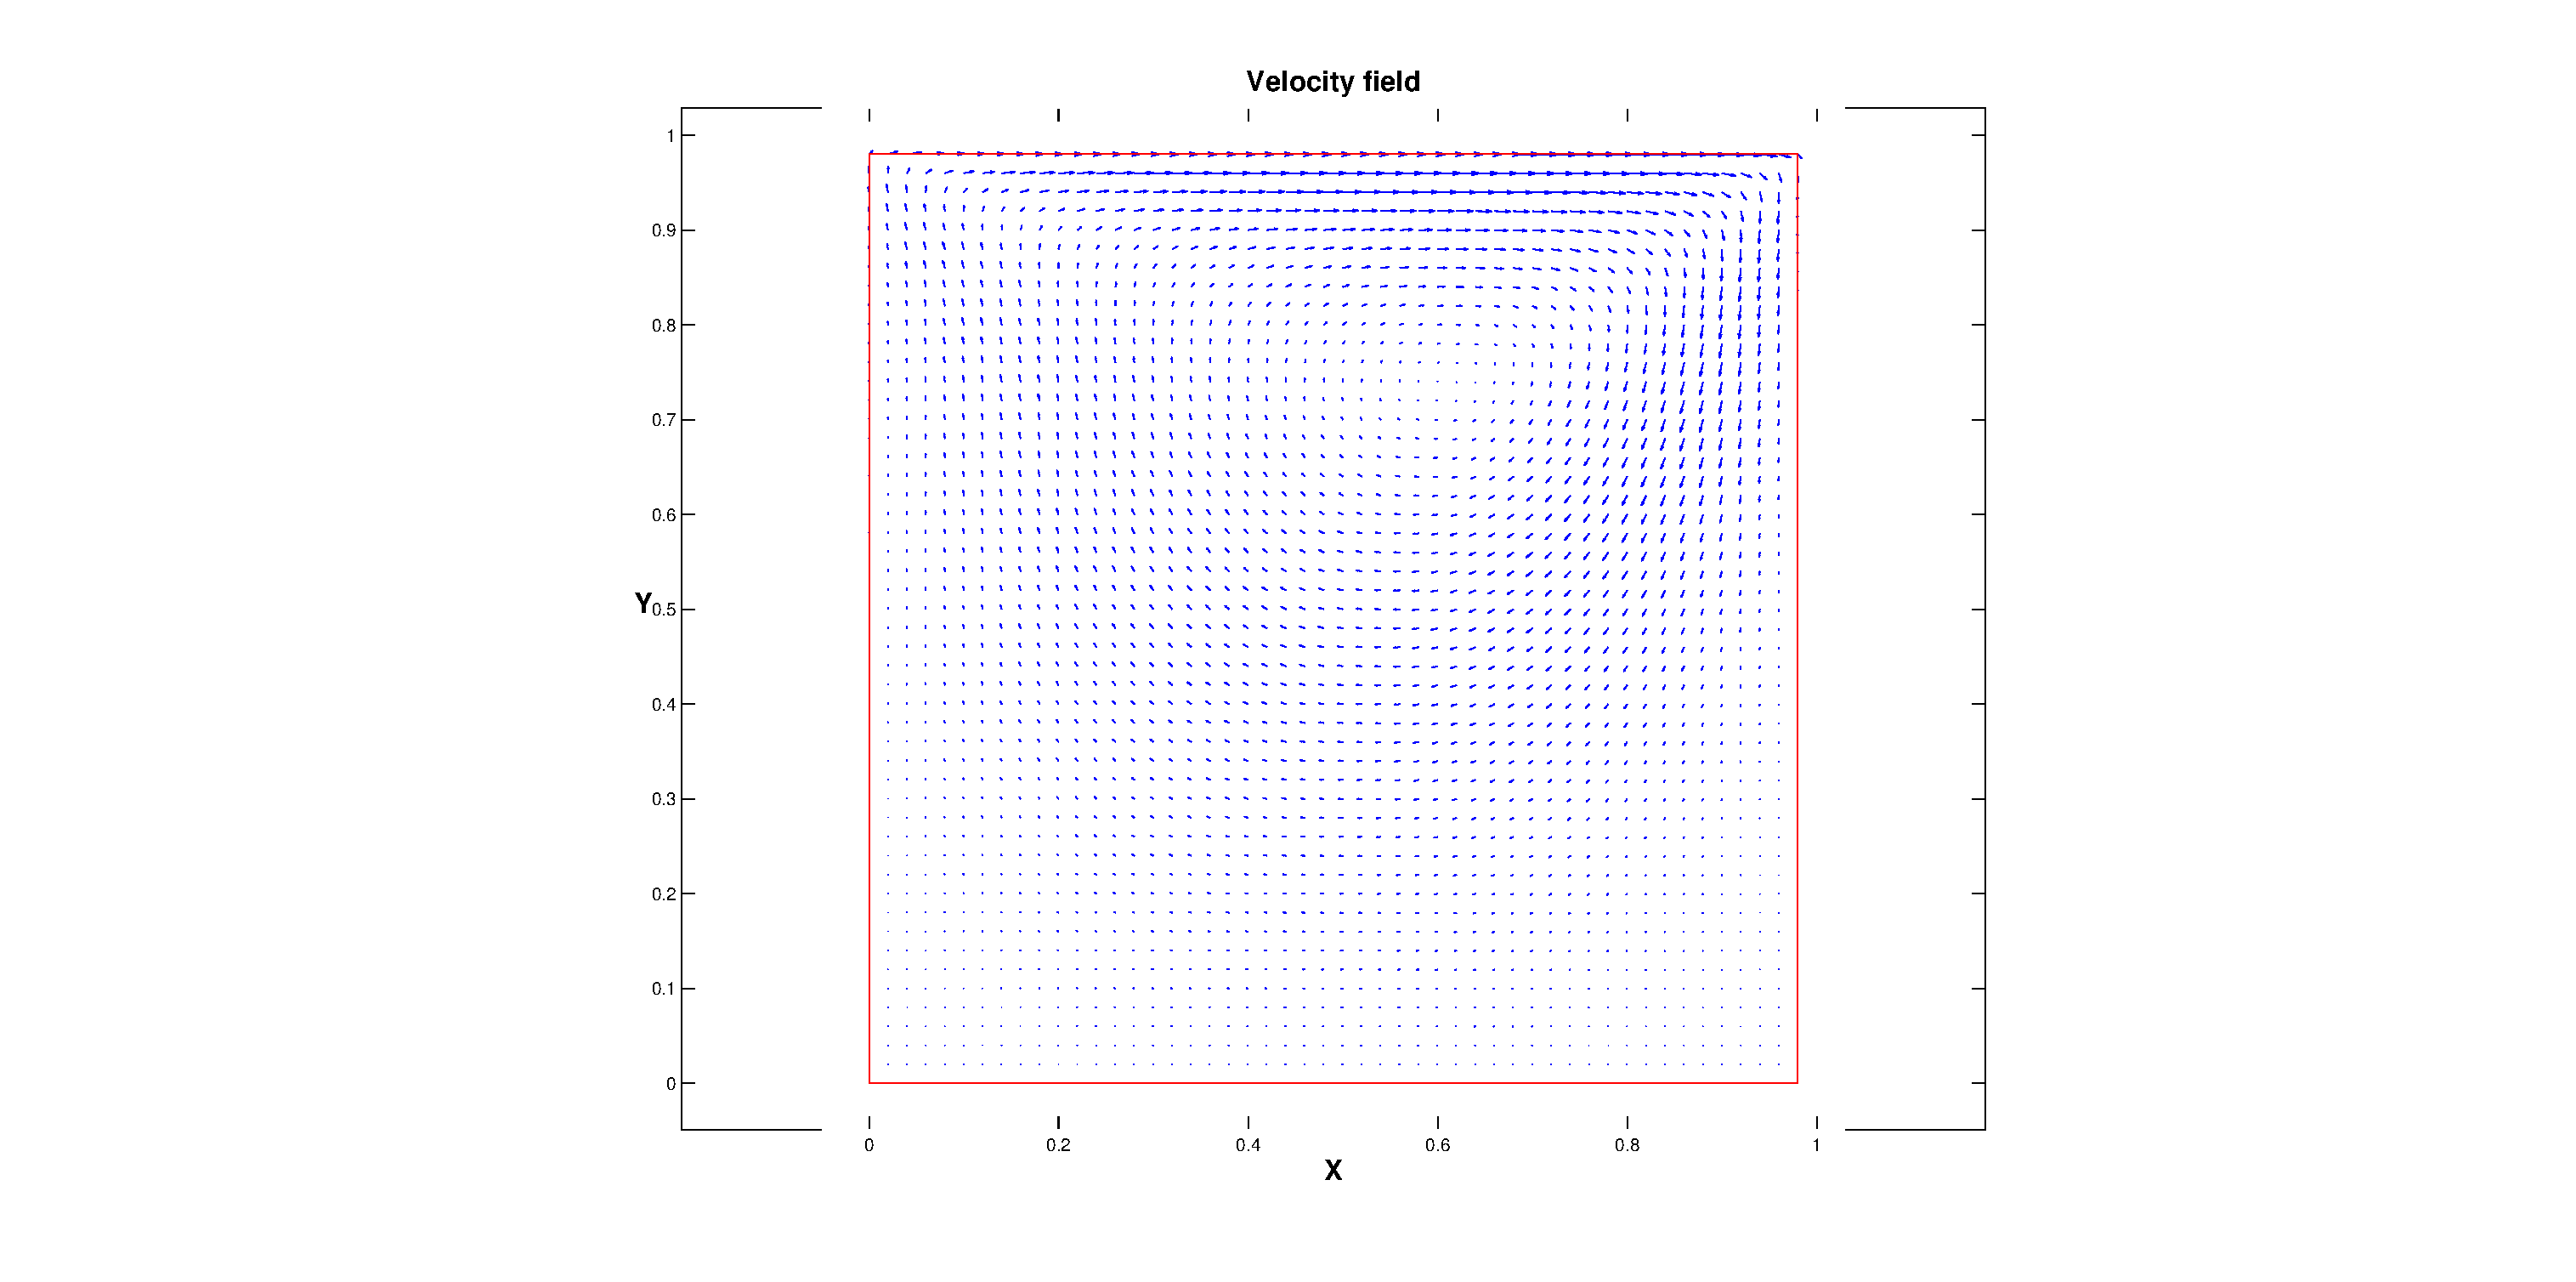
\includegraphics[scale = .3]{dcavity_velocityfield}
\end{slide}


\begin{slide}[Dissolve]{Flow Over a Backward-Facing Step Cont.}
\begin{center}
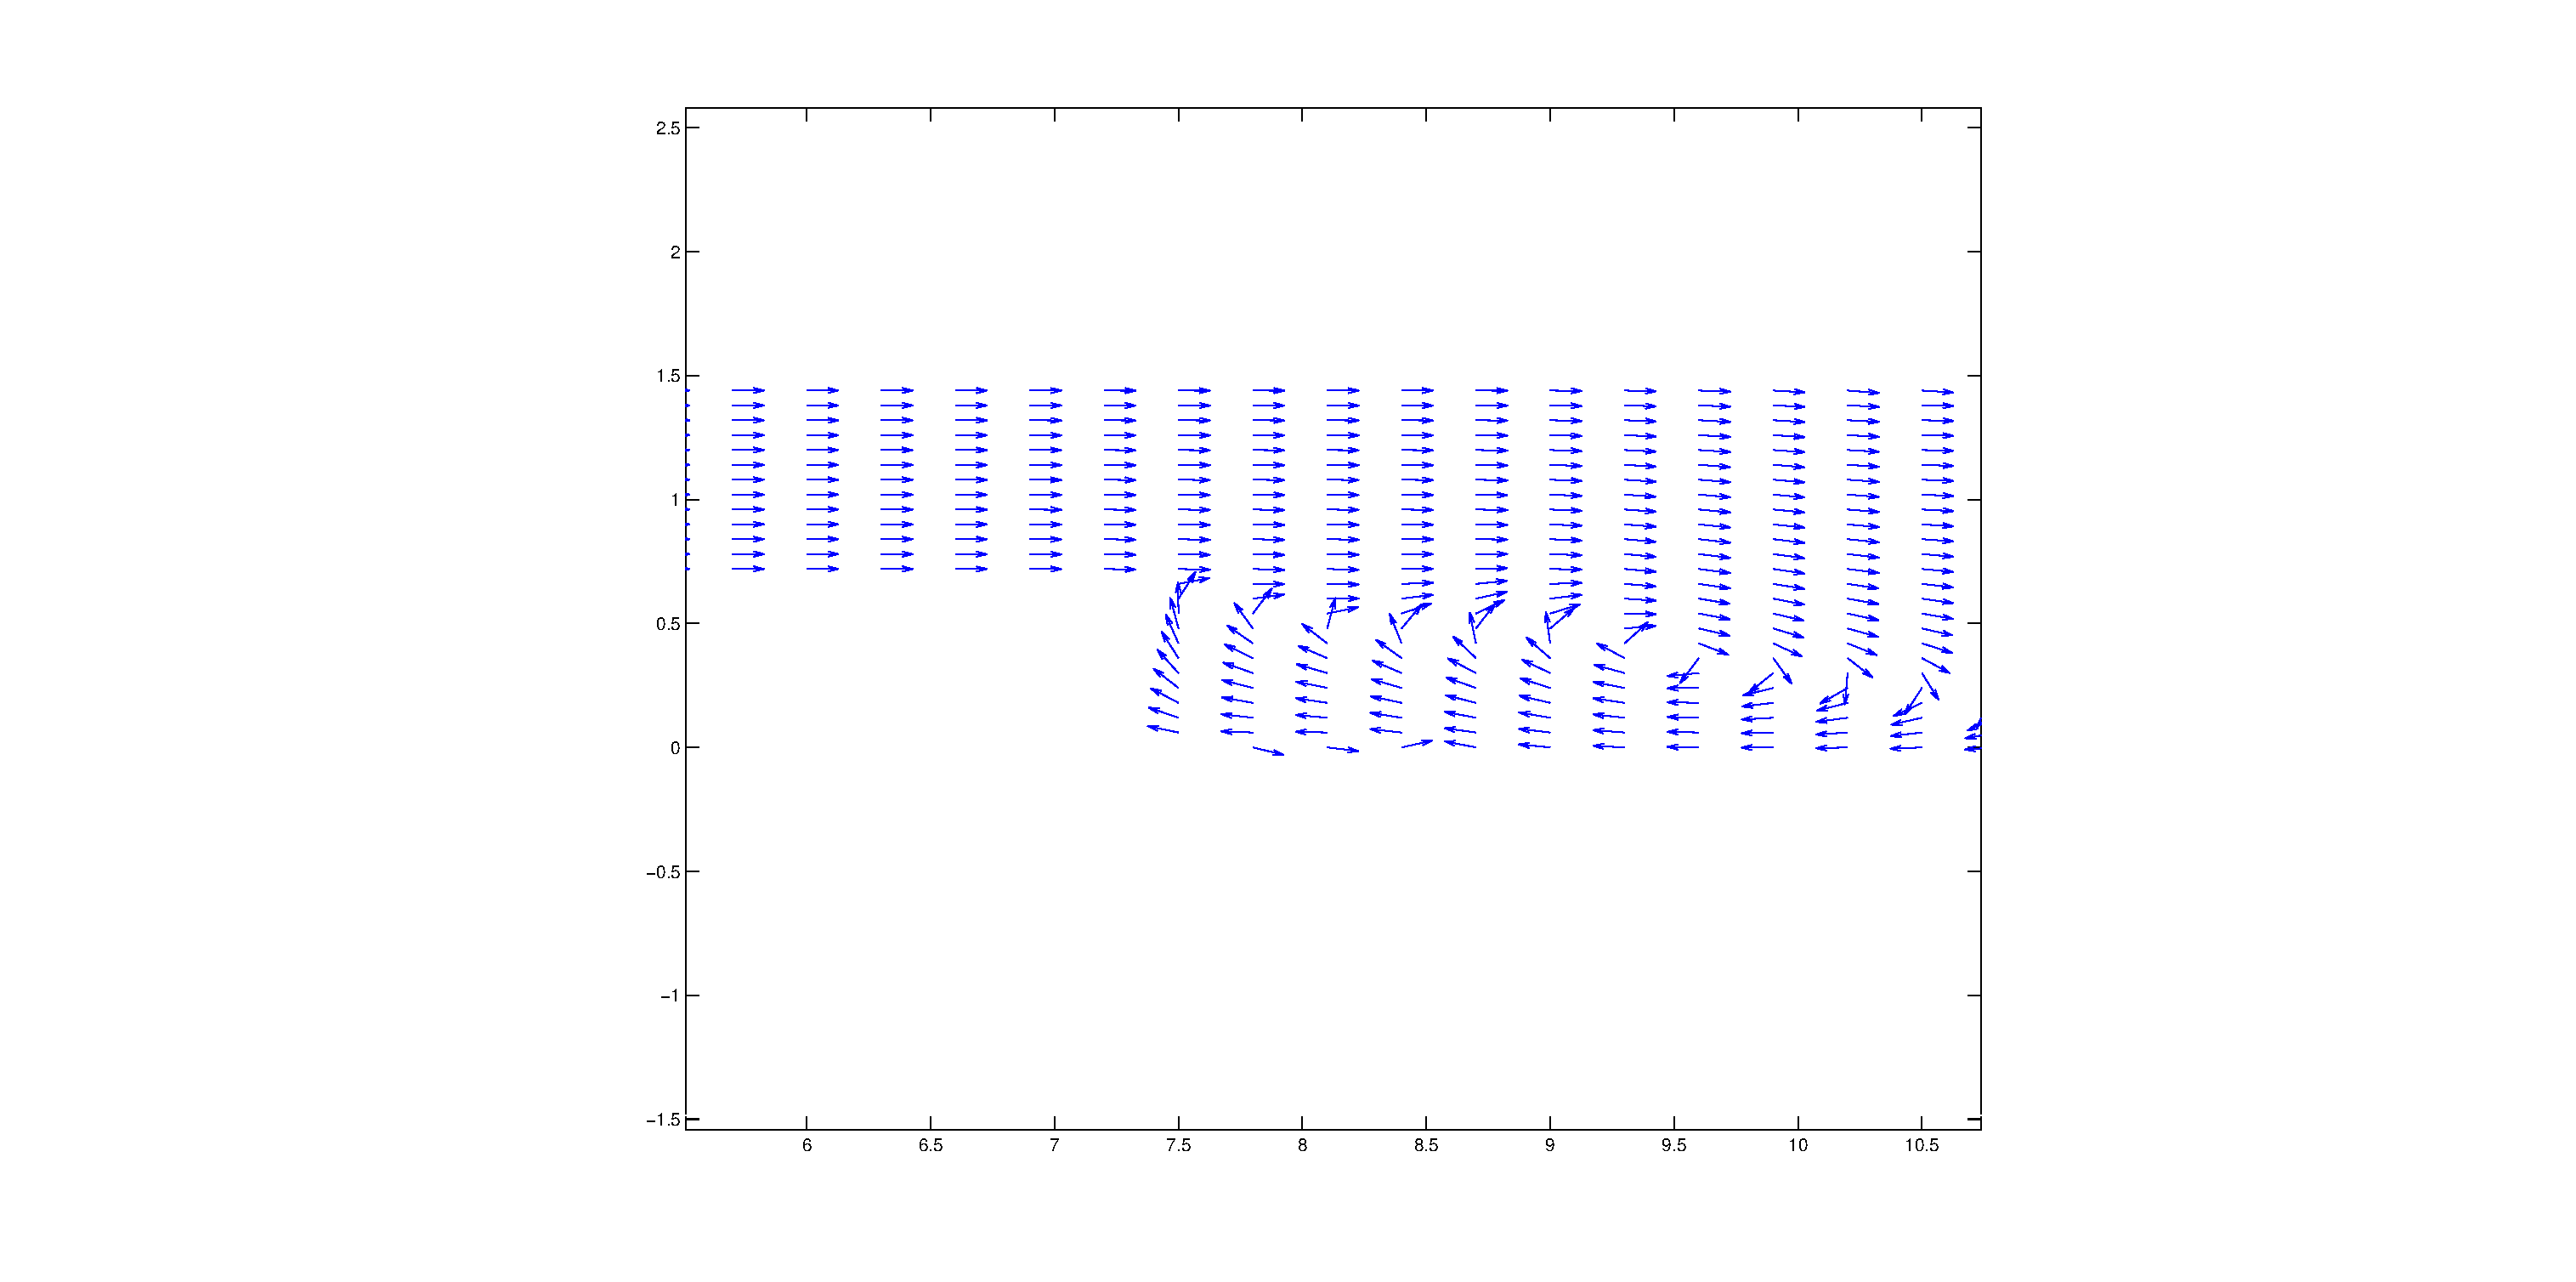
\includegraphics[scale = .3]{backstep_velocityfield_t10}
\end{center}
\end{slide}


\begin{slide}[Dissolve]{Flow Over a Backward-Facing Step}
\begin{center}
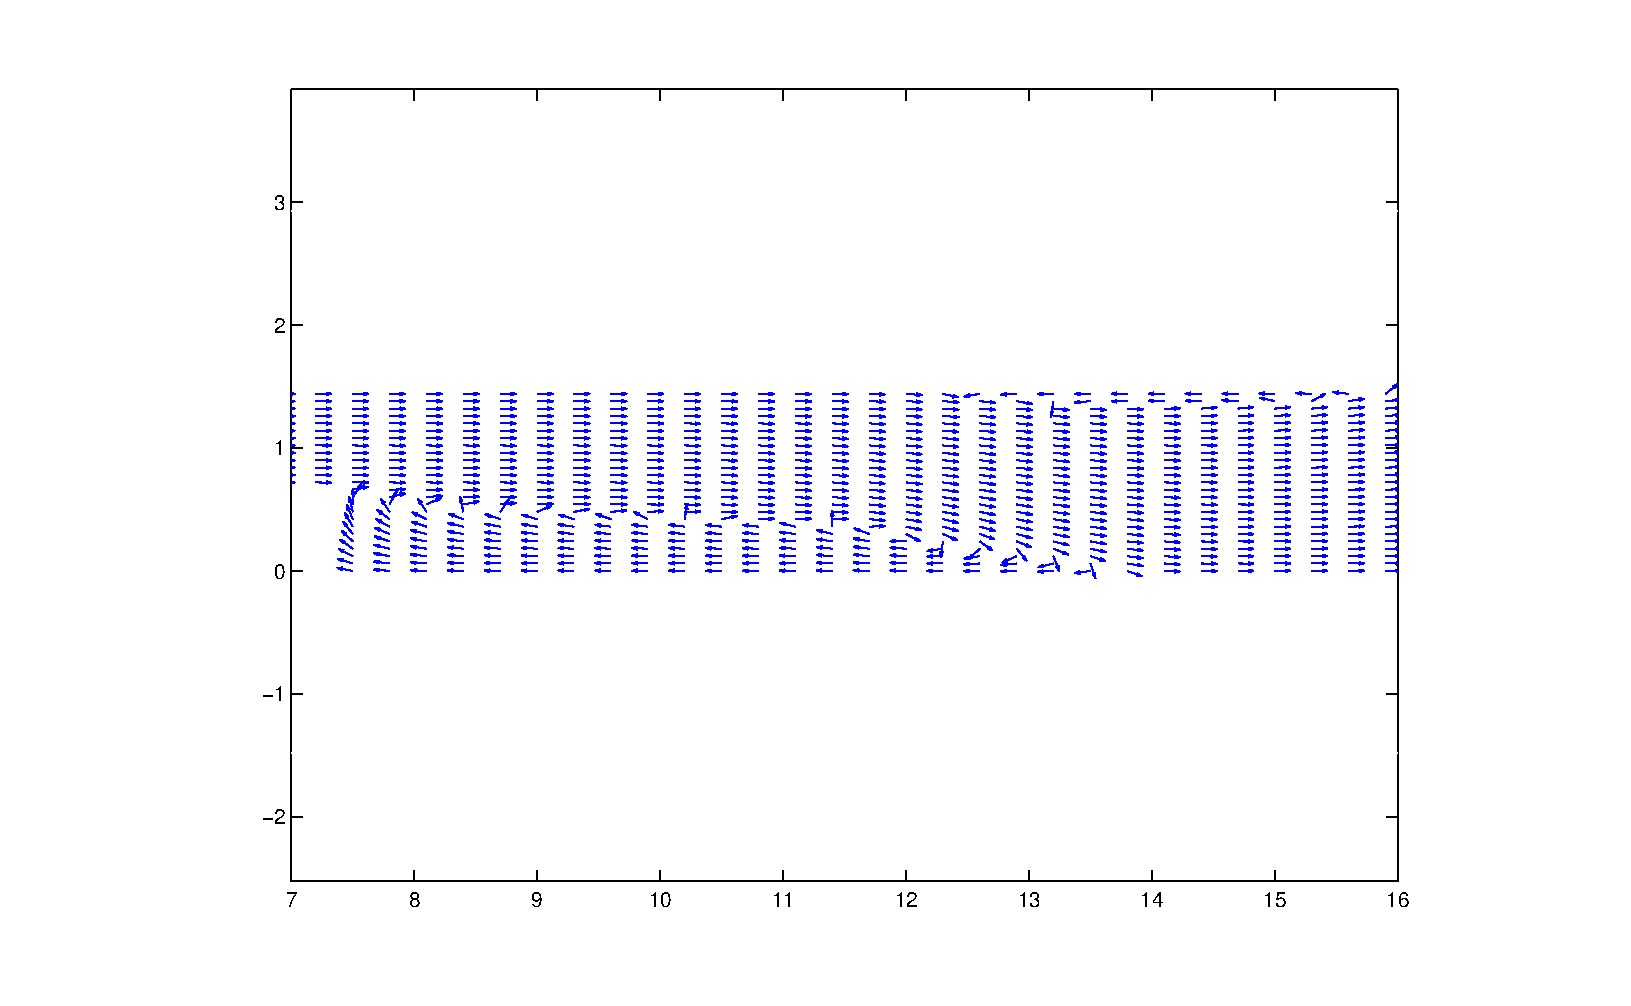
\includegraphics[scale = .4]{backstep_velocityfieldfinal}
\end{center}
\end{slide}

\begin{slide}[Dissolve]{Flow Past an Obstacle}
\begin{center}
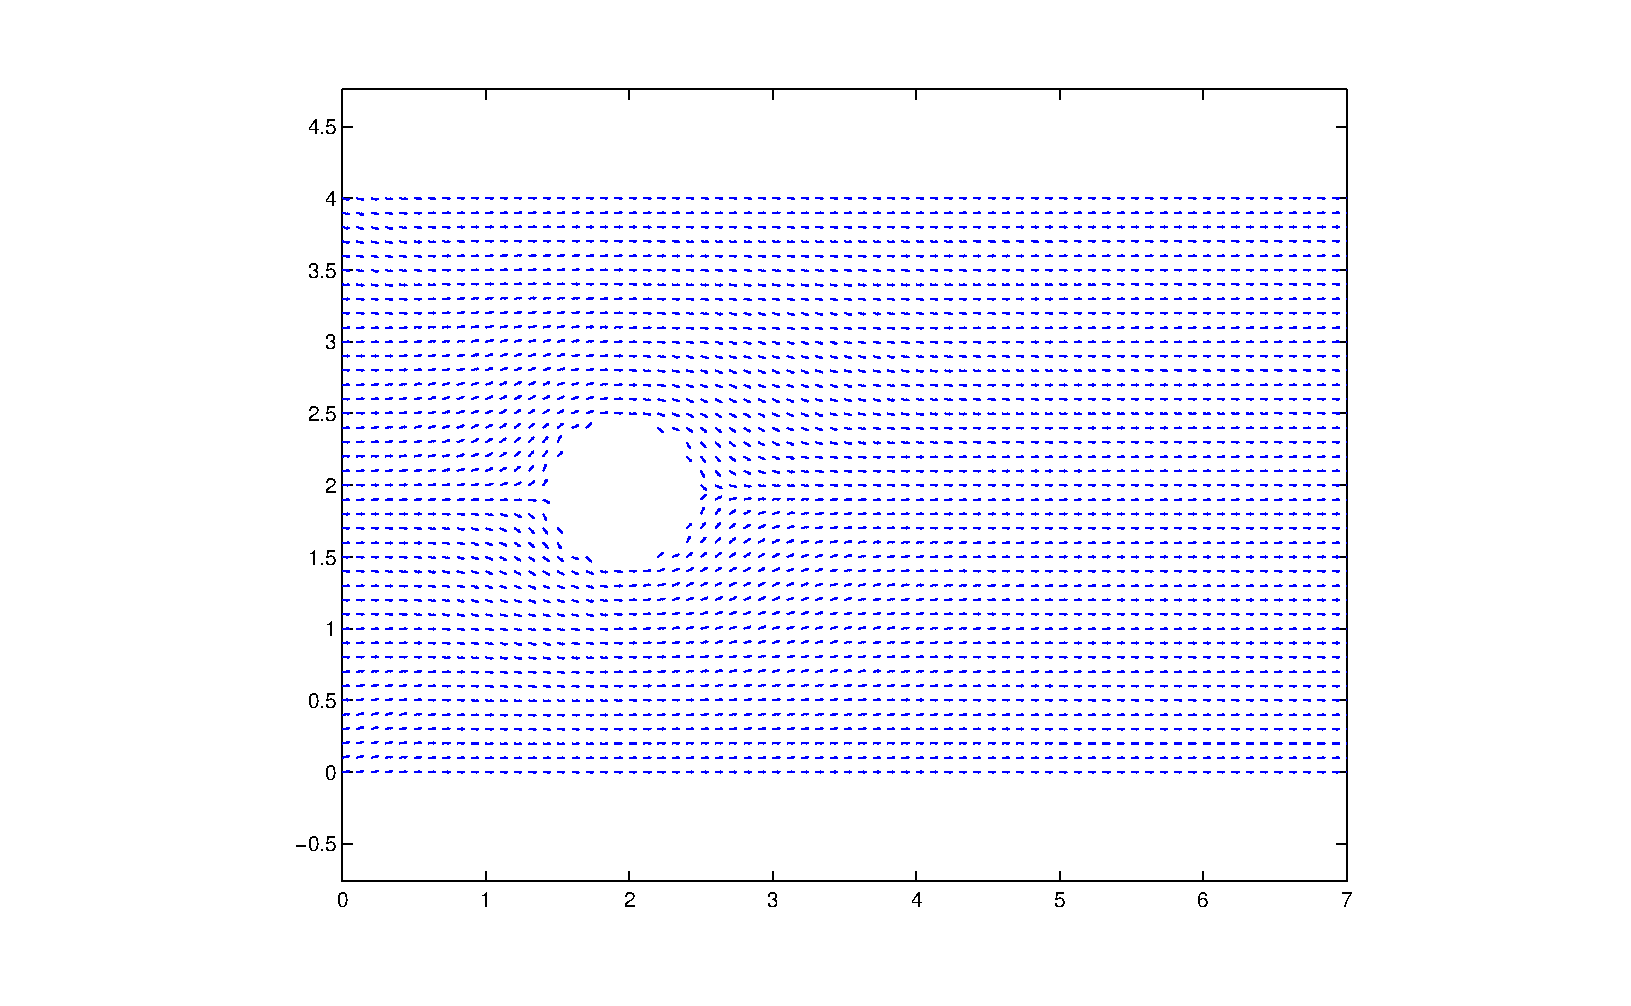
\includegraphics[scale = .4]{circle}
\end{center}
\end{slide}

\begin{slide}[Dissolve]{Flow Past an Obstacle}
\begin{center}
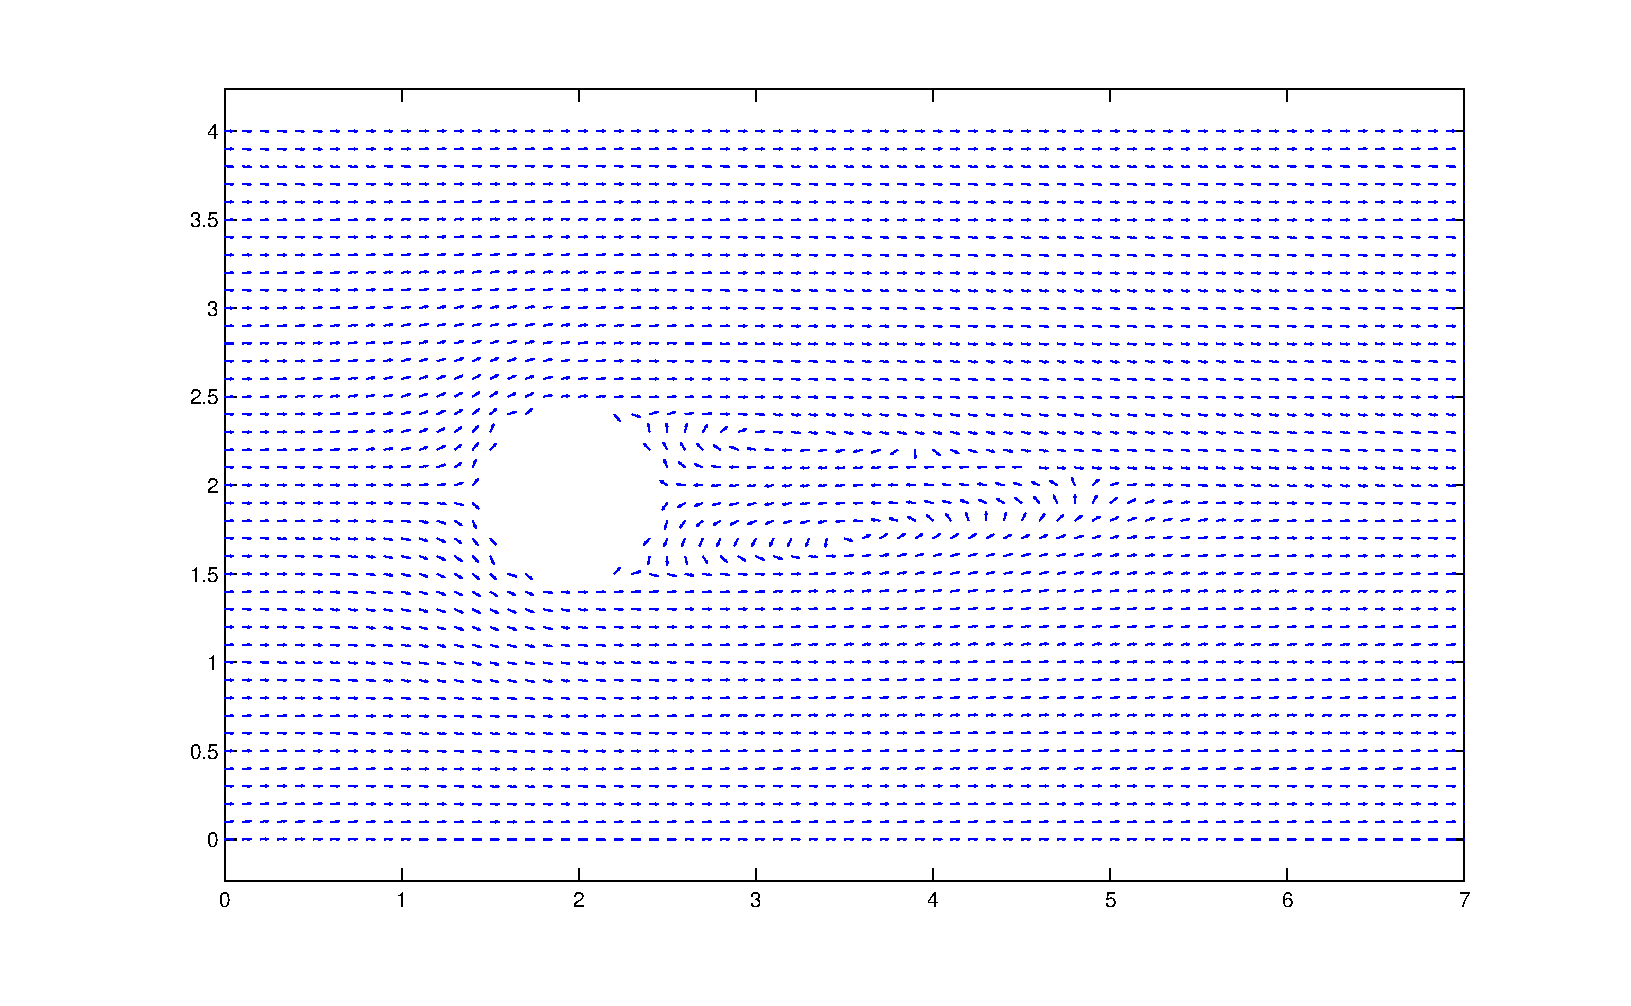
\includegraphics[scale = .4]{circle100}
\end{center}
\end{slide}

\end{document}